Following section describes the options available for dimensioning drawings and how to use them. eCAD provides range of dimensioning tools which can be used to quickly dimension any drawing. eCAD divides dimensions into three main categories: Horizontal, Vertical, Diametric Radial. The first two options are for dimensioning lines and the next two are for the circles/arcs. These options are available in the menubar under the Dimension menu.
\subsection{Horizonatal Dimensioning} 
To start with, just create a drawing. So let's start
\begin{enumerate}
\item Click File and then New. Save the File.
\item The first thing is to draw a simple object so that we can dimension it. Let us draw a square.
\item Select Horizontal from the Dimension menu.
\item Move the cursor over either the left top point or bottom left point of your
square and click once.
\item Now move the cursor horizontally to the right to the right edge of the square
and click once.
\item Without clicking the mouse move the line up or down a you will notice the
dimension appears. You can now place it where you want to and when you are
satisfied click one time to set it.
\begin{figure}[h!]
\centering
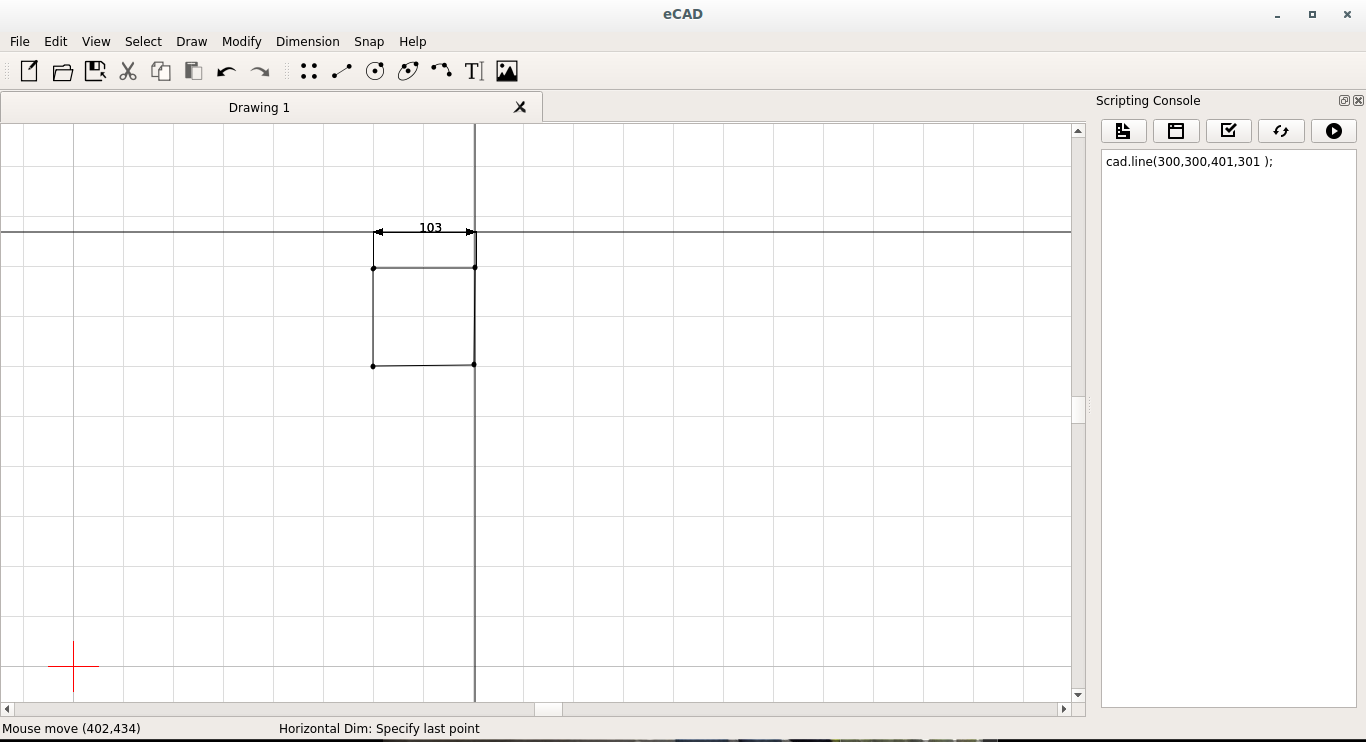
\includegraphics[width=0.8\textwidth]{images/hdim.png}
\end{figure}
\end{enumerate}
\subsection{Vertical Dimensioning}
You may follow the steps below for vertical dimensioning. We will dimension the above drawn square now vertically
\begin{enumerate}
\item Select Vertical from the Dimension menu.
\item Select upper left point of the square and click once.
\item Move the cursor vertically downwards and click once the bottom left point of the square.
\item Without clicking move your mouse to the right and the vertical dimension.
appears. Move it where your want it and click once and now you have dimensioned the square.
\begin{figure}[h!]
\centering
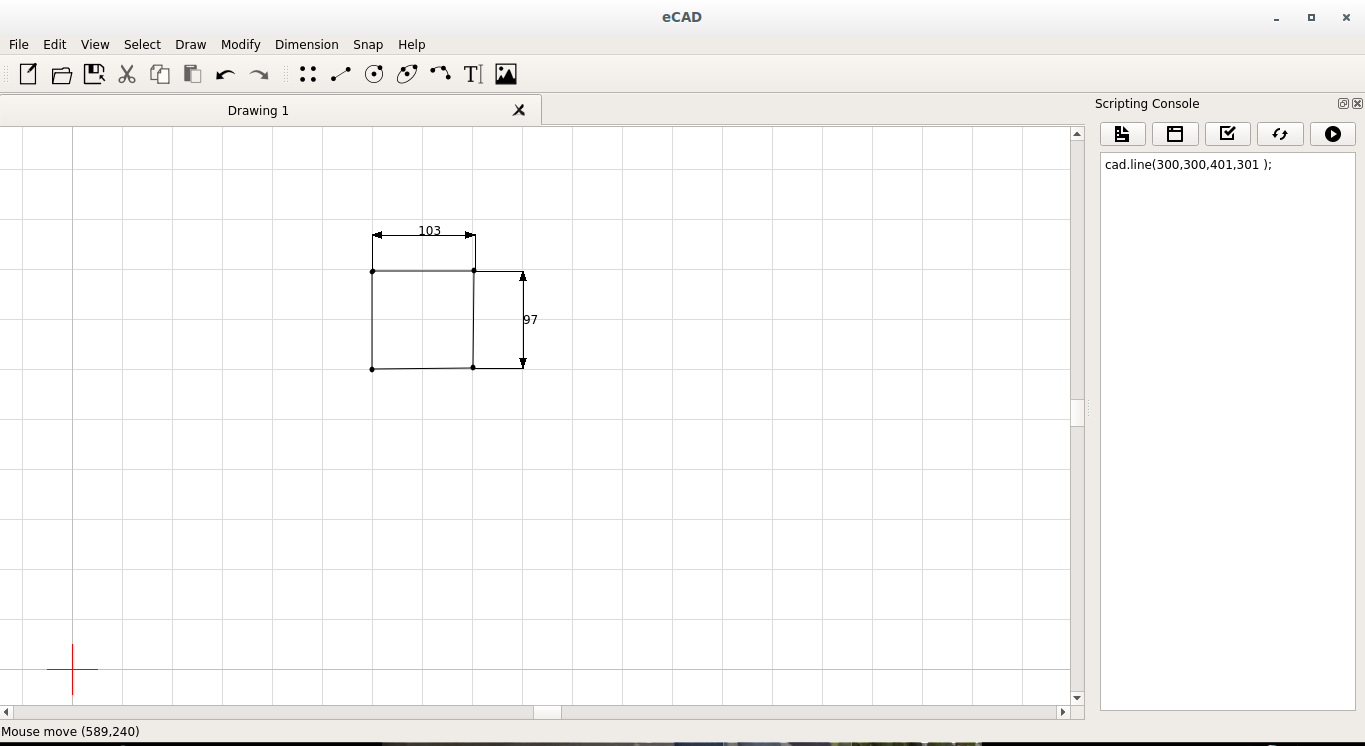
\includegraphics[width=0.8\textwidth]{images/vdim.png}
\end{figure}
\end{enumerate}
\subsection{Radial Dimensioning}
Begin by drawing a circle.
\begin{enumerate}
\item Select Dimension and click Radial from the Dimension Menu.
\item Touch the edge of the circle with your cursor and click once.
\item Without clicking your mouse, move it away from the circle. Notice the
dimension appears. Now move the around the circle and you will see the
dimension moves around the circle. Pick a spot you want your dimension and
click once.
\begin{figure}[h!]
\centering
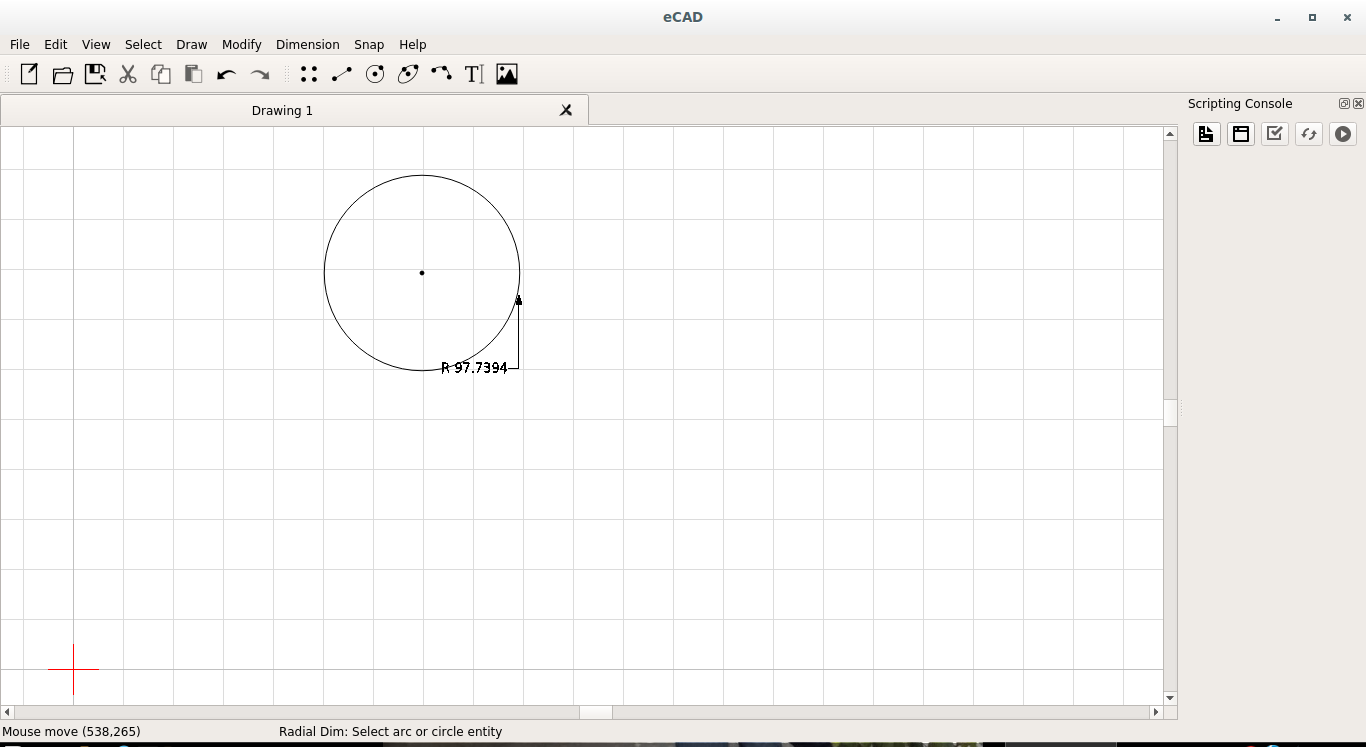
\includegraphics[width=0.8\textwidth]{images/radial.png}
\end{figure}
\end{enumerate}
\subsection{Diametric Dimensioning}
It Creates diametric dimensions for circle or arc entities and similarly set the position of the diametric dimension line using the mouse.
